\documentclass[tikz,border=5pt]{standalone}
\usepackage{pgfplots}
\pgfplotsset{compat=1.18}

\definecolor{corba}{HTML}{3F51B5}
\definecolor{referencia}{HTML}{6B7280}

\begin{document}
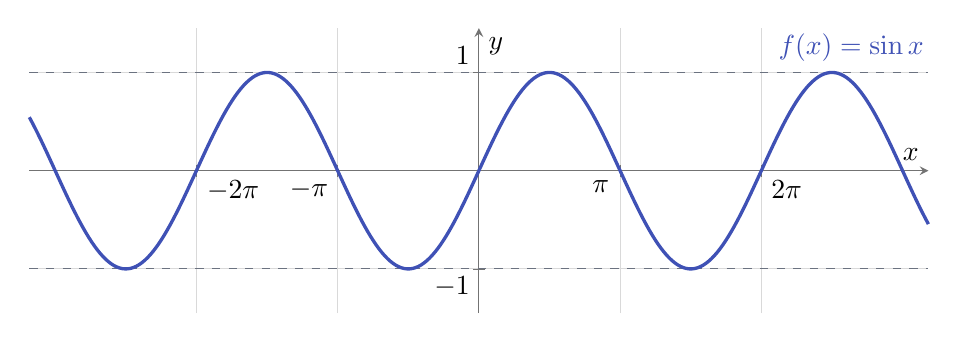
\begin{tikzpicture}
  \begin{axis}[
    width=13cm,
    height=5.2cm,
    axis lines=middle,
    xmin=-10,
    xmax=10,
    ymin=-1.45,
    ymax=1.45,
    xlabel={$x$},
    ylabel={$y$},
    xtick={-6.2832,-3.1416,0,3.1416,6.2832},
    xticklabels={{},{},$0$,{},{}},
    ytick={-1,1},
    yticklabels={{},{}},
    axis line style={black!55},
    tick style={black!55},
    grid=major,
    grid style={black!15},
    clip=false,
  ]
    \addplot[referencia, dashed, domain=-10:10] {1};
    \addplot[referencia, dashed, domain=-10:10] {-1};
    \addplot[corba, very thick, domain=-10:10, samples=320] {sin(deg(x))};
    \node[corba, anchor=south east, inner sep=1.5pt]
      at (axis cs:10,1.06) {$f(x)=\sin x$};
    % Cada etiqueta va al costat on la corba no la travessa
    \node[anchor=north west, inner sep=1.5pt] at (axis cs:-6.15,-0.05) {$-2\pi$};
    \node[anchor=north east, inner sep=1.5pt] at (axis cs:-3.25,-0.05) {$-\pi$};
    \node[anchor=north east, inner sep=1.5pt] at (axis cs:3.0,-0.05) {$\pi$};
    \node[anchor=north west, inner sep=1.5pt] at (axis cs:6.4,-0.05) {$2\pi$};
    \node[anchor=south east, inner sep=1.5pt] at (axis cs:-0.1,1.03) {$1$};
    \node[anchor=north east, inner sep=1.5pt] at (axis cs:-0.1,-1.03) {$-1$};
  \end{axis}
\end{tikzpicture}
\end{document}
